\documentclass[11pt,a4paper]{book}

\usepackage{Appunti}

\begin{document}
\title{Clean Coder\\
\large{\textit{Robert C. Martin}}}
\author{Jacopo De Angelis}
\maketitle

\pagebreak
\tableofcontents
\pagebreak

\chapter{Professionalità}
\section{Prendere le proprie responsabilità}
Come si può "imparare" a prendersi le proprie responsabilità? Ci sono alcuni principi da seguire.

\section{Non fare del male}
Come può un programmatore fare del male? Può farlo al software, creando problemi per le funzioni e alla struttura del software.
\subsection{Non danneggiare la funzionalità}
Chiaramente il software deve funzionare, non solo per noi programmatori ma anche per clienti e datori di lavoro. Per essere professionali, insomma, non bisogna creare bug.
\begin{figure}[h!]
	\begin{center}
		
\includegraphics[scale=0.3]{img/001.jpg}
		\caption{Tu in questo momento}
		\label{fig: 001}
	\end{center}
\end{figure}
Il concetto è che quello deve essere l'impegno di un programmatore e nel caso escano dei bug deve prendersene la responsabilità se causati dal proprio codice.

\subsubsection{I QA non dovrebbero trovare niente}
Qual è il codice per il quale non sai se i QA\footnote{Quality assurance, coloro incaricati di testare il codice} troveranno qualcosa? Il codice di cui non si è certi.

Usare i QA come dei cacciatori di bug rende il processo più lungo e riduce la fiducia nei programmatori. Mandare in testing codice di cui non si è sicuri è violare la regola del "non fare del male".

I QA troveranno errori nel codice? Probabile.

\subsection{Devi sapere che funziona}
Come? Semplice, testando il codice.\\
Paura di metterci troppo? Automatizzali scrivendo degli unit test.\\
Quanto codice andrebbe testato? Tutto.\\
Come fare? Automatizzarli tramite suite di test.

\subsection{Non danneggiare la struttura}
In breve: devi poter fare cambiamenti senza dover ribaltare l'intera struttura.

Il problema è che in certi casi i progetti non sono estremamente flessibili e non permettono questo agio nelle modifiche. I design pattern sono qualcosa che solitamente vengono applicati pedissequamente ma una cosa da ricordare è che per una piattaforma flessibile dobbiamo essere anche noi stessi flessibili.

Quindi come fare? Quando si scopre che il codice non è così semplice da modificare allora si modifica il design per rendere più semplici i cambiamenti successivi\footnote{Belle parole se il codice non è composto da oltre 60k linee di codice}.

Un programmatore professionale cambierà il nome di un metodo o di una classe senza troppi problemi se lo riterrà necessario.\footnote{Quando si lavora in un gruppo di una certa magnitudine un cambiamento del genere rischia di essere deleterio però, è vero che gli strumenti di refactoring sono diventati più potenti ma le convenzioni di nome e di codice ci sono per un motivo.}

\subsection{Etica lavorativa}
Un programmatore è responsabile della propria educazione e del proprio miglioramento, non è un compito da affidare al datore di lavoro. Se esso aiuta con questo percorso meglio, è gentile, ma non è una sua responsabilità.

NDR: Il libro qua fa dei calcoli riguardo il tempo da dedicare al lavoro e quanto da dedicare al tempo per lo studio individuale. Non mi addentrerò in questi esempi perchè considero abbastanza sciocco fare calcoli sul tempo altrui. Propongo la lettura di \href{https://muldoon.cloud/programming/2020/04/17/programming-rules-thumb.html}{questo articolo} invece. Credo che sia più importante ricordare alle persone che non serve essere il migliore sulla piazza certe volte, magari le proprie priorità sono differenti. Non ho assolutamente nulla contro chi vuole arrivare a quei livelli, anzi, faccio loro i complimenti, ma è meglio non dimenticare che in quanto esseri umani non viviamo solo per lavorare, abbiamo anche altre passioni magari, o altri desideri. Impariamo a coltivare anche quelli. Sempre lavorare al massimo delle proprie capacità ma non per forza uccidersi dallo stress per essere i migliori in assoluto.

\subsection{Conoscere il tuo campo}
\textit{"Do you know what a Nassi-Schneiderman chart is? If not, why not? Do you
know the difference between a Mealy and a Moore state machine? You should.
Could you write a quicksort without looking it up? Do you know what the term
“Transform Analysis” means? Could you perform a functional decomposition
with Data Flow Diagrams? What does the term “Tramp Data” mean? Have you
heard the term “Conascence”? What is a Parnas Table?"}

Secondo Martin queste cose andrebbero conosciute da un programmatore. Ci terrei a precisare che probabilmente sono cose che ha imparato tramite lavoro, trovandosi davanti a nuovi problemi e nuove soluzione. Non è una colpa non conoscere qualcosa, è una colpa non voler imparare davanti ad una lacuna.

\subsection{Collaborazione}
Il secondo migliore modo per imparare è collaborare con gli altri. Un professionista si sforza per programmare in gruppo.

\subsection{Insegnamento}
Il miglior modo per imparare è farlo sapendo di doverlo spiegare ad altri.

\subsection{Conoscere il proprio dominio}
Lavori su di un programma di contabilità? Allora dovresti conoscere il campo della contabilità. Programma per agenzie di viaggi? Conoscenza dell'industria dei viaggi.

\subsection{Identificare il proprio datore di lavoro/cliente}
I problemi del tuo datore di lavoro sono i tuoi problemi. Devi dimostrare di comprendere quali essi siano e lavorare verso la loro migliore soluzione.

\subsection{Umiltà}
Per riassumere questo paragrafo: sii un buon essere umano. Sii cosciente delle tue capacità ma sentiti pronto a metterti in dubbio e fare domande. Non sapere qualcosa non è una vergogna, è normale certe volte doversi aggiornare o essere messi in questione.

Non ridicolizzare o sminuire gli altri.

\chapter{Dire di no}
\section{Ruoli avversari}
Ruoli avversari non vuol dire arrivare a puntare le lame al collo dell'altro, vuol dire che i vari attori delle discussioni hanno degli interessi lavorativi personali (far uscire il prodotto subito, sviluppare bene le funzionalità, ecc.). Un ruolo avversario positivo è quello nel quale le due parti difendono i propri interessi e cercano di trovare una soluzione nel mezzo che possa soddisfare tutti il più possibile, insomma, una soluzione pareto efficiente.

\subsection{E riguardo al perchè?}
"Fatti, non pugnette". Il perchè è meno importante del crudo fatto la maggior parte delle volte. In più spesso dare troppe spiegazioni può portare l'altro a pensare di poter gestire la cosa (e no, non in un senso da "e allora fallo tu", ma più da "quindi ora mi dici cosa fare?").

\section{Alto rischio}
Il momento migliore per dire no è quando il rischio è più alto.

\section{Sapere fare gruppo}
Un buon lavoratore in squadra comunicare frequentemente, aiutare e farsi aiutare dai colleghi, svolgere le proprie mansioni in maniera diligente. Non è colui che dice sì ogni volta.

\subsection{Provarci}
Dire "ok, ci proverò" è il peggior servizio che tu possa fare a chiunque sia coinvolto nella discussione a lavoro. "Provarci" ha vari significati in base alla parte che deve interpretare la parola; per alcuni sarà un "ce la farò", per altri un dare il contentino ma mentire spudoratamente, in certi casi si potrebbe intendere nella maniera più letterale possibile eppure si lascerebbe troppo spazio all'incertezza.

\subsection{Aggressività passiva}
Qua una delle parti più difficili: cosa fare quando ci si trova davanti ad un qualcuno che sta agendo contro gli interessi del gruppo. Si potrebbero creare prove (fondate ovviamente) che la comunicazione è sempre avvenuta in maniera trasparente in modo da parare le spalle al gruppo e permettere all'altro di fregarsi da solo o, e forse è meglio, cercare di risolvere di propria mano il problema che sta venendo creato prima del tracollo. Insomma, avvisare tutti che il treno sta arrivando e di spostarsi e filmarsi per dire di avere le prove del fatto o andare direttamente dalle persone, urlando, mettendosi a rischio, dicendo di spostarsi?

\section{Il costo di dire sì}
\href{http://raptureinvenice.com/?p=63}{Lettura consigliata nel libro}, spiega molto bene cosa voglia dire "dire sì senza pensarci" e il perchè certa gente meriti legnate sui denti.

\section{Codice impossibile}
Dopo aver letto il racconto si può evincere una cosa: dire no è importante. John avrebbe dovuto dire no alla deadline di due settimane, poi all'aggiunta di funzioni, poi al lavoro straordinario. 

Dire no è importante per noi stessi e anche per il datore di lavoro.

\chapter{Dire di sì}
\section{Il linguaggio dell'impegno}
Di'. Intendilo. Fallo.
\begin{enumerate}
	\item Tu dirai che lo farai
	\item Tu intenderai veramente ciò
	\item Tu lo farai effettivamente
\end{enumerate}

\subsection{Riconoscere la mancanza di impegno}
Secondo Martin ci sono alcune parole chiave che mostrano la mancanza di impegno:
\begin{itemize}
	\item Dovrei: "dovrei fare ciò", "dovrei perdere peso", "qualcuno dovrebbe farlo"
	\item Spero: "Spero di finire entro domani", "spero che ci incontreremo nuovamente", "spero di avere tempo per ciò"
	\item Plurale maiestatis: "incontriamoci qualche volta", "finiamo il lavoro"
\end{itemize}

\subsection{Il suono dell'impegno}
Prima pensa a cos'è effettivamente sotto il tuo controllo e poi impegnati.
\begin{figure}[h!]
	\begin{center}
		
\includegraphics[scale=0.3]{img/001.jpg}
		\caption{Tu in questo momento}
		\label{fig: 0012}
	\end{center}
\end{figure}
\footnote{Sì, nuovamente la stessa ma ehi, l'ha chiamata}.
La parola che compare più spesso quando qualcuno decide di mettere il proprio impegno in qualcosa è "io (più le sue varie declinazioni)" e poi una frase riguardante lo svolgimento di un compito. Secondo l'autore è impossibile svincolarsi da una dichiarazione d'impegno tale.
\begin{figure}[h!]
	\begin{center}
		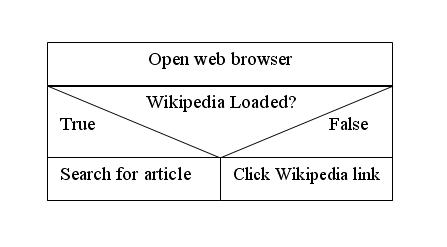
\includegraphics[scale=0.45]{img/002.jpg}
		\caption{Questa sezione è un bellissimo meme, vero?}
		\label{fig: 002}
	\end{center}
\end{figure}

Scherzi a parte, è il concetto di analizzare cosa tu sia effettivamente in grado di fare e dire che farai ciò, non cose a caso, non belle speranze.

Ecco alcune ragioni per le quali non si potrebbe intendere veramente
\subsubsection{Non funzionerebbe perchè dipendo da persona X per farlo}
Puoi fare promesse solo su ciò che controlli al 100\%.

\subsubsection{Non funzionerebbe perchè non so se possa effettivamente essere fatto}
Se non sai se X possa essere fatto, puoi dire che ti impegnerai nei passi che conducono a X.

\subsubsection{Non funzionerebbe perchè non farei in tempo}
Possono accadere cose per le quali non si può più raggiungere un certo traguardo, in quel caso è meglio avvisare subito. Se, a causa del traffico, stai arrivando in ritardo ad un appuntamento, avvisa.

\section{Come dire sì}
Fondamentalmente:
\begin{itemize}
	\item non mentire
	\item contratta
	\item spiega le tue riserve
	\item valuta solo se veramente necessario cosa bisogna fare in più, rubando tempo alla propria vita, e chiedi una compensazione per ciò, che sia tempo libero o soldi
\end{itemize}

\chapter{Scrivere codice}
Sei stanco? Non scrivere codice. Il codice scritto da stanchi è probabilmente pieno di errori di logica, non pulito, non connesso.

Non entrare in uno stato catatonico nel quale ti senti produttivo perchè solitamente ti trovi solo a scrivere codice che non testi, o codice che pensa ad un solo caso e non a tutti, non refattorizzato ecc.

La musica? Qua l'autore svela di avere fatto cose pessime ascoltando musica, non è una regola generale, se ti senti concentrato va benissimo, non isolarti in maniera assoluta però, la musica deve rilassarti, non isolarti.

Blocco dello scrittore? Cerca qualcuno con cui scrivere in coppia. Capita di avere un blocco, può derivare da tantissimi fattori.

Se sei stanco e non riesci a concentrarti o se ti stai ossessionando su di un dettaglio stacca, non cambia niente nel tuo ragionamento se continui a sbatterci la testa.

Capita a tutti di essere in ritardo, tutti.

Qualcuno vuole aiutarti? Accetta. La persona non sta aiutando veramente? Dopo un po' gentilmente falli tornare al loro posto. C'è qualcuno che puoi aiutare? Aiutarlo. Insomma, sii un buon essere umano.

\chapter{Test Driven Development (TDD)}
\section{Le tre leggi del TDD}
\begin{enumerate}
	\item Non puoi scrivere codice in produzione se non hai scritto prima un test che fallisca
	\item Non puoi scrivere altri unit test rispetto a quelli sufficienti e non compilare è un fallimento
	\item Non puoi scrivere altro codice in produzione rispetto a quello sufficiente per far passare i test
\end{enumerate}

\section{I benefici}
\subsection{La certezza}
Avere tanti test non è sbagliato, anzi, è un'ottima cintura di sicurezza. Appena si cambia qualcosa nel codice basta eseguire i test e possiamo sapere immediatamente se abbiamo rotto qualcosa o no.

In più se vuoi modificare una funzione per renderla più efficiente ma hai paura di rompere qualcosa, i test diventano la tua rete di sicurezza.

\chapter{Acceptance testing}
Prima di tutto: tutti vorrebbero sapere subito precisamente cosa ci sarà da fare e come farlo. Realtà: impossibile.

C'è sempre un elemento di incertezza in stime e proposte.

Una delle prime cose da ricordare è che nell'ambiguità si creano problemi. Quando si risponde su supposizioni e non certezze si rischia di creare un problema per il futuro.

\section{Acceptance test}
Un acceptance test è quello che viene scritto assieme agli stakeholders per decidere quando un requisito è completato.

\subsection{Definition of done}
Ci sono svariate definizioni in base alle aziende, una definizione usata comunemente è "è finito quando il codice è scritto, passa i test, QA e gli stakeholders hanno accettato".

\subsection{Automazione}
I test di accettazione dovrebbero essere sempre automatizzati, controllare e testare ogni volta costa. Tanto.

I test andrebbero fatti dalle BU e dai QA, non sempre è così purtroppo. Il ruolo dello sviluppatore è testare il sistema con i nuovi AT e vedere come vada.

Ricordiamo una cosa: gli acceptance test non sono unit test. I secondi sono scritti dai programmatori per i programmatori. I primi sono scritti dal business per il business. 

E per le GUI? Meglio creare un sistema di API sotto da testare rispetto al creare delle chiamate all'interfaccia.

\chapter{Strategie di testing}
\href{https://github.com/JacopoDeAngelis/Appunti-vari/blob/master/Testing/Testing.pdf}{Qua} un pratico riassunto.
\section{QA}
I QA non dovrebbero trovare nulla ma dopotutto il loro lavoro è anche il pensare in maniera non normale, troveranno sempre qualcosa.

Sono parte del team, non sono avversari.

Sono coloro i quali scrivono le vere specifiche e i veri requisiti per il sistema.

Sono quelli che si occupano del \href{http://www.satisfice.com/articles/what_is_et.shtml}{testing esplorativo}.

\section{La piramide del testing}
\begin{figure}[h!]
	\begin{center}
		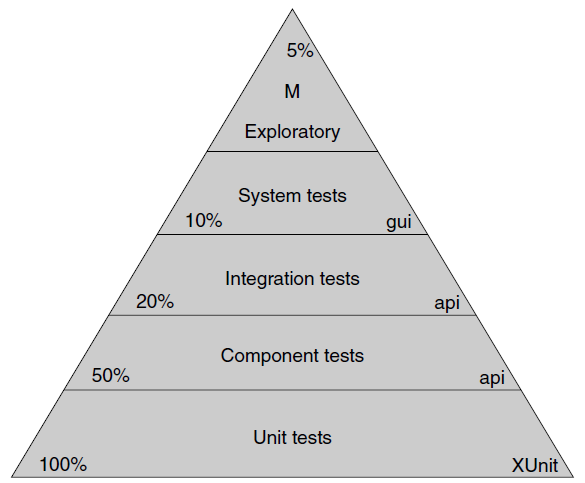
\includegraphics[scale=0.6]{img/003.png}
		\caption{Piramide del testing}
		\label{fig: 003}
	\end{center}
\end{figure}

\subsection{Unit test}
Questi test servono per testare il sistema al livello più basso e in maniera atomica. Sono eseguiti ad ogni ciclo di CI\footnote{Continuous Integration}.

La loro copertura dovrebbe essere del 100\%.

\subsection{Component test}
Un component test si occupa di passare dei dati ad un component e leggere l'output. SI utilizza un sistema di mocking per rendere l'unità isolata dal resto in modo da testare solo essa.

\subsection{Integration test}
Non testano il codice, testano come tutto sia coordinato correttamente tra i vari elementi.

\subsection{Test di sistema}
Controllano che nell'esperienza utente tutto sia dove deve essere.

\subsection{Esplorazione manuale}
Qua è quando gli esseri umani decidono di spaccare tutto e farlo venendo pagati. I tester per ciò non sono nostri nemici, non è vero che "ah, chi mai farebbe una cosa del genere" perchè se c'è qualcosa che internet ha insegnato è che la gente ogni tanto si diverte anche solo a creare problemi.

\chapter{Gestione del tempo}
\section{Meeting}
I meeting sono essenziali e sono anche potenzialmente una perdita di tempo. Non serve andare a tutti gli incontri se questi non sono necessari come non è necessario rimanere fino alla fine se non è più richiesto il proprio input.

\subsection{Stand up}
Semplici incontri di quindici minuti dove si deve dire:
\begin{itemize}
	\item cosa si è fatto ieri
	\item cosa si farà oggi
	\item che problemi sono stati incontrati
\end{itemize}

Basta, eventuali discussioni saranno per il post riunione

\subsection{Planning}
Sono incontri nei quali si spiegano i nuovi requisiti e in gruppo si stima quando può richiedere in giorni uomo.

Si discute anche del backlog degli sviluppatori e se rifiutarle o continuarle.

\subsection{Retrospective e demo}
Si esegue alla fine di ogni sprint e serve per vedere cosa è andato bene, cosa male e cosa si può fare per migliorarlo.

\subsection{Discussioni}
Discutere richiede sangue freddo e preparazione. Qualcuno deve gestirlo in certi casi e le parti devono arrivare documentando in maniera seria il proprio caso, non solo cercando di imporsi.

\chapter{Stime}
\subsection{Cos'è una stima?}
Una stima è un'idea, non è un impegno strettamente parlando. Mancare una stima non è un disonore, possono essere successe cose nel frattempo.

Quando viene chiesta una stima questa è accompagnata sempre da una percentuale di incertezza, non sai bene se ce la farai, la tua stima è sì ma probabilmente sai anche che possono esserci rallentamenti di vario tipo.

\subsection{Stima PERT}
In questo sistema vengono richieste tre stime:
\begin{itemize}
	\item O: stima ottimista, ovvero il caso nel quale tutto vada perfettamente
	\item N: stima nominale, ovvero quella più probabile
	\item P: stima pessimista, ovvero quella nel caso qualcosa vado male
\end{itemize}

Possiamo quindi descrivere la stima con due formule:
$$\mu=\dfrac{O+4N+P}{6}$$
questa è la durata attesa del compito
$$\sigma=\dfrac{P-O}{6}$$
Questa è la deviazione standard, è la misura dell'incertezza della stima.

\section{Stimare un compito}
Spesso una stima non è eseguita da una sola persona ma dal team.
\subsection{Metodo wideband delphi}
Il gruppo si riunisce, discutono, stimano e discutono sulle stime fino al raggiungimento di un consenso.

Un sito comodo per eseguire queste stime nel team durante una chiamata è \href{https://www.planningpoker.com/}{Planningpoker}. Per quanto riguarda i numeri da inserire per le stime è meglio dare un range fisso in modo da non potersi scostare di troppo e poter analizzare le deviazioni in gruppo. Ad esempio si può usare la serie di Fibonacci per dare alcuni numeri standard su cui convergere.

\chapter{Pressione}
\section{Evitare la pressione}
Il miglior modo per rimanere calmi è evitare le situazioni stressanti.
\begin{figure}[h!]
	\begin{center}
		
\includegraphics[scale=0.4]{img/004.jpg}
		\caption{Ormai non serve nemmeno l'immagine completa}
		\label{fig: 004}
	\end{center}
\end{figure}

\subsection{Impegno}
Come abbiamo visto nel capitolo precedente non ci si deve impegnare per stime che sono, per l'appunto, stime.

In certi casi ci troviamo di fronte a promesse non fatte da noi, in quel caso non siamo tenuti ad onorare le promesse che non abbiamo fatto.

\subsection{Pulizia}
Non personale\footnote{Anche se quella non guasta} ma del codice. Non bisogna cercare di velocizzare il lavoro creando problemi nel codice perchè comunque questi creeranno rallentamenti successivamente.

\subsection{Gestione delle crisi}
Scegli delle linee guida che rispetteresti in un momento di crisi e rispettale sempre, non solo quando ci sono problemi.

\section{Gestire la pressione}
\begin{enumerate}
	\item Non panicare: panicare non risolve niente
	\item Affidati alla tua disciplina
	\item chiedi aiuto se non riesci a risolvere qualcosa
\end{enumerate}

\chapter{Collaborazione}
Una cosa che dobbiamo sempre ricordarci è che lavorare con altre persone non è un qualcosa che deve darci problemi, le convenzioni sociali e aziendali esistono e nessuno può pensare di essere superiore ad esse. Comprenderle, accettarle e comprendere il proprio spazio di manovra è ciò che può aiutarci a non rendere un ambiente di lavoro ancora più confuso e, certe volte, stressante di quanto non sia già.

Bisogna imparare a lavorare in gruppo anche e non pensare che il proprio codice non possa mai essere modificato. I programmi evolvono, i requisiti anche.

\chapter{Gruppi e progetti}
Non pensare che un programmatore possa occuparsi di due progetti differenti contemporaneamente e che questi siano "magicamente seguiti in maniera perfetta". Non esiste dedicare tot tempo a uno e tot all'altro.

I team devono essere creati e bisogna lasciare del tempo affinchè essi si mischino, cementino e crescano.

\chapter{Insegnamento, apprendimento e arte}
Nessuno nasce imparato e chi fa "gatekeeping" della professione è presto destinato a lavorare da solo. Coloro i quali hanno più esperienza dovrebbero assumere un ruolo di aiuto, insegnamento verso chi viene dopo e chi invece è nel proprio viaggio di apprendimento (anche appena iniziato) deve accettare che è normale non sapere e che la migliore disposizione sia quella del volere apprendere.

\end{document}